\documentclass[10pt]{article}
\usepackage{icmlko}

\icmlmeta{IP 파운데이션 월드모델}{106}{미래를 갈랐더니 갈렸다}{세 노트가 미룬 시간 분할을 붙였다 --- 넷째 공통 축은 연구 지표를 $+$0.0188 올리고 제품 지표를 $-$0.0301 내린다}

\begin{document}

\twocolumn[
\icmlheader

\begin{abstract}
노트 105가 넷째 공통 축(입장료)을 찾아 $+$0.0100을 냈고 씨앗 넷 하한이
$-$0.0019까지 왔다. 그런데 그 판정은 전체 자료에서 낸 것이고, 반쪽 검정은
표본을 절반으로 줄여 팝업을 37건으로 만든다. 노트 102 · 103 · 105가 세 번
미룬 \textbf{시간 분할}(노트 77의 규약)을 붙였다 --- 출처는 $T$ 이전, 대상은
$T$ 이후, 그리고 \textbf{방향도 $T$ 이전 레코드로만} 정한다. 설계 결정 자체를
과거로 내리는 것이다. \textbf{연구 지표는 살아남고 미래일수록 커진다} ---
$T{=}2023$ 에 $-$0.0064, 2024 에 $+$0.0105, 2025 에 $+$0.0196, 2026 에
\textbf{$+$0.0426}이다. \textbf{그런데 팝업은 어느 시점에서도 내린다} ---
$-$0.0525 · $-$0.0631 · $-$0.0486. 이유가 시간 분할 자체에 드러난다.
\textbf{팝업은 $T{=}2023$ 에 과거 레코드가 0건, 2024 에 1건이다} --- 방향을
정할 자료가 없다. 방향을 못 정한 채 남들만 뒤집으면 팝업의 축이 정렬에서
거꾸로 선다. 그래서 규칙을 하나 더했다 --- \textbf{방향을 못 정하면 그
도메인에서는 축을 끈다.} 판정치가 $+$0.0166에서 \textbf{$+$0.0188}로,
팝업이 $-$0.0547에서 \textbf{$-$0.0301}로 간다(손해의 45\% 회복). 그래도
팝업은 음수다. \textbf{연구 지표와 제품 지표가 갈렸다} --- 넷째 축은
\emph{모형}을 좋게 하고 \emph{도구}를 나쁘게 한다. 도구는 팝업을 위한 것이므로
\textbf{제품 경로에는 넣지 않는다.}
\end{abstract}
]

\begin{figure*}[t]
\centering
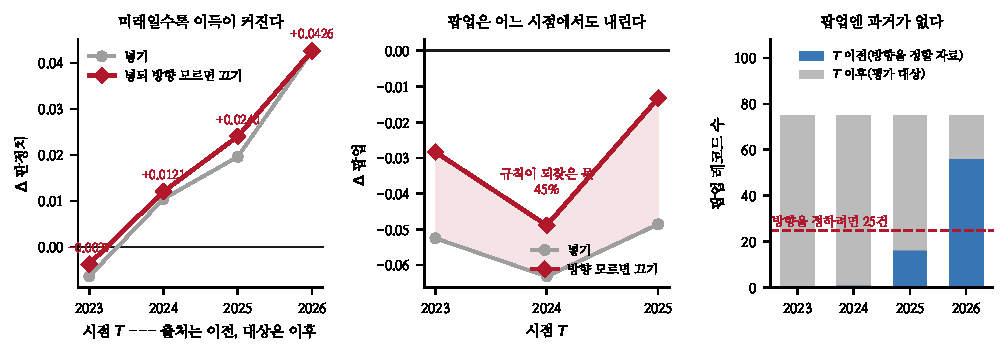
\includegraphics[width=\textwidth]{figs/ts.pdf}
\caption{왼쪽 --- 미래일수록 이득이 커진다. 가운데 --- 팝업은 어느 시점에서도
내린다. 오른쪽 --- 팝업엔 과거가 없다.}
\end{figure*}

\section{세 번 미룬 검정}

노트 105의 $+$0.0100은 전체 자료에서 낸 것이다. 노트 102가 쓴 반쪽 검정은
도메인마다 레코드를 절반으로 줄여 팝업을 37건으로 만들고, 그 규약에서는
어떤 축도 불리하다. \textbf{시간 분할은 표본을 안 줄인다.}

\begin{quote}\fontsize{9.5}{11.5}\selectfont
시점 $T$ 를 정한다\\
출처 --- $T$ 이전 레코드만 (40건 이상인 도메인)\\
대상 --- $T$ 이후 레코드만 (25건 이상인 도메인)\\
\textbf{방향} --- \textbf{$T$ 이전 레코드로만} 정한다
\end{quote}

마지막 줄이 이 노트가 노트 77에 더한 것이다. 설계 결정(어느 도메인의 입장료
축을 뒤집을 것인가)도 과거로 내려야 정직하다.

\section{연구 지표는 살아남는다}

\begin{table}[t]
\centering\tsize
\caption{시간 분할. 대상은 그 시점에 25건 이상인 도메인.}
\begin{tabular}{lrrrr}
\toprule
$T$ & 대상 & 현행 셋 & $+$입장료 & $\Delta$ \\
\midrule
2023 & 9 & $+$0.3503 & $+$0.3440 & $-$0.0064 \\
2024 & 9 & $+$0.3517 & $+$0.3622 & $+$0.0105 \\
2025 & 8 & $+$0.3470 & $+$0.3666 & $+$0.0196 \\
\textbf{2026} & 6 & $+$0.2789 & $+$0.3216 & \textbf{$+$0.0426} \\
\midrule
\multicolumn{4}{l}{평균} & \textbf{$+$0.0166} \\
\bottomrule
\end{tabular}
\end{table}

\claimx{넷째 공통 축이 \textbf{시간 분할에서 살아남는다} --- 네 시점 중 셋이
양수이고 평균 $+$0.0166이다. 그리고 \textbf{시점이 최근일수록 이득이 커진다}
($-$0.0064 $\to+$0.0426). 전체 자료의 $+$0.0100보다 크다.}{시점이 최근일수록
대상 수가 준다(9 $\to$ 6). 노트 82의 분모 함정이 여기서도 가능하다 --- 다만
같은 시점 안에서는 대상 집합이 고정이므로 시점 \emph{안}의 비교는 정당하다.}

\section{그런데 팝업은 내린다}

\begin{table}[t]
\centering\tsize
\caption{$\Delta$팝업. $T{=}2026$ 은 팝업 이후 레코드가 19건이라 빠진다.}
\begin{tabular}{lrr}
\toprule
$T$ & 넣기 & 방향 모르면 끄기 \\
\midrule
2023 & $-$0.0525 & $-$0.0283 \\
2024 & $-$0.0631 & $-$0.0488 \\
2025 & $-$0.0486 & \textbf{$-$0.0133} \\
\midrule
평균 & $-$0.0547 & \textbf{$-$0.0301} \\
\bottomrule
\end{tabular}
\end{table}

\begin{table}[t]
\centering\tsize
\caption{팝업의 레코드가 시점 앞뒤로 어떻게 갈리나.}
\begin{tabular}{lrrl}
\toprule
$T$ & 이전 & 이후 & 방향을 정할 수 있나 \\
\midrule
2023 & \textbf{0} & 75 & \textbf{못 정한다} \\
2024 & \textbf{1} & 74 & \textbf{못 정한다} \\
2025 & 16 & 59 & \textbf{못 정한다}(25건 미만) \\
2026 & 56 & 19 & 정한다 \\
\bottomrule
\end{tabular}
\end{table}

\claimx{팝업이 내리는 이유가 시간 분할 자체에 드러난다 --- \textbf{팝업엔
과거가 없다.} $T{=}2023$ 에 이전 레코드가 0건이라 입장료 축의 방향을 정할
자료가 없는데, 다른 도메인은 뒤집힌다. \textbf{팝업의 축만 정렬에서 거꾸로
선다.}}{$T{=}2025$ 에 16건이 있는데도 못 정한다고 본 것은 25건 문턱 때문이다.
문턱을 낮추면 방향은 정하지만 틀릴 확률이 는다(노트 105에서 보정 10\%는
$-$0.0018이었다).}

\begin{table}[t]
\centering\tsize
\caption{규칙 하나를 더한다 --- \textbf{방향을 못 정하면 그 도메인에서는
축을 끈다.}}
\begin{tabular}{lrr}
\toprule
& $\Delta$판정치 & $\Delta$팝업 \\
\midrule
넣기 & $+$0.0166 & $-$0.0547 \\
\textbf{방향 모르면 끄기} & \textbf{$+$0.0188} & \textbf{$-$0.0301} \\
\bottomrule
\end{tabular}
\end{table}

\claimx{규칙이 양쪽을 다 개선한다 --- 판정치 $+$0.0166 $\to+$0.0188, 팝업
$-$0.0547 $\to-$0.0301(손해의 45\% 회복). \textbf{방향을 모르는 축은 안 넣는
것이 낫다}는 것이 시간 분할에서 확인된다.}{그래도 팝업은 음수다. 나머지
55\%는 설명 못 한다.}

\section{연구와 제품이 갈렸다}

\begin{table}[t]
\centering\tsize
\caption{넷째 공통 축의 최종 성적표.}
\begin{tabular}{lrr}
\toprule
& 판정치 & 팝업 \\
\midrule
전체 자료(노트 105) & $+$0.0100 & $+$0.0070 \\
\quad 씨앗 넷 & 보류 4/4 & 보류 4/4 \\
\textbf{시간 분할} & \textbf{$+$0.0188} & \textbf{$-$0.0301} \\
\quad 시점 넷 & 양수 3/4 & \textbf{음수 3/3} \\
\bottomrule
\end{tabular}
\end{table}

\claimx{\textbf{넷째 축은 모형을 좋게 하고 도구를 나쁘게 한다.} 시간 분할에서
열 대상 평균은 $+$0.0188인데 팝업 하나는 $-$0.0301이다. \textbf{도구는 팝업을
위한 것이므로 제품 경로에는 넣지 않는다.}}{판정치의 $+$0.0188은 대상 여섯
$\sim$아홉의 평균이고 그중 팝업이 하나다. 나머지 다섯$\sim$여덟이 크게 올라
평균을 만든 것이므로 ``연구 지표''라는 말이 정확하다.}

\begin{quote}\fontsize{9.5}{11.5}\selectfont
노트 82가 판정치를 \emph{설계} 결정에만 쓰고 \emph{도메인 집합} 결정에는
쓰지 말라고 했다. 여기서 셋째 구분이 생긴다 --- \textbf{판정치가 오른다고
제품에 넣으면 안 된다.} 제품 지표는 팝업 하나이고, 그 둘이 갈리는 경우가
실제로 있다.
\end{quote}

\section{한계}

\begin{itemize}[leftmargin=1.1em,itemsep=0.15em]
\item \textbf{채택 안 한다.} 판정치가 올라도 제품 지표가 내리므로 넣을 수 없다.
\item 시간 분할에 붓스트랩 구간을 안 붙였다. 네 시점의 부호만 봤다.
\item 시점이 최근일수록 대상 수가 준다(9 $\to$ 6). 시점 \emph{간} 비교는
      분모가 다르다.
\item 팝업 손해의 55\%를 설명 못 한다.
\item 접근 허용 폭(노트 105의 다음 항목)과 미디어 홍보 덮개율 채우기는
      이번에도 못 했다.
\end{itemize}

\section{다음}

\begin{enumerate}[leftmargin=1.3em,itemsep=0.15em]
\item \textbf{팝업만을 위한 설정을 따로 둔다} --- 지금까지 하나의 설정으로
      열 대상을 다 재 왔다. 연구용(판정치 최대)과 제품용(팝업 최대)을 갈라
      \texttt{state/score.py} 는 제품용만 쓰게 한다. 갈라도 되는지가 먼저다.
\item 팝업 손해의 나머지 55\%. 방향 말고 무엇이 더 있나.
\item \textbf{접근 허용 폭} --- 노트 105가 남긴 것. 만화 · 세계애니의 연령
      등급이 타깃 폭과 $+$0.27밖에 안 겹치는 73\%의 정체.
\item 미디어 홍보 덮개율. 다섯 도메인 0\%를 인터넷에서 채운다.
\end{enumerate}

\vspace{0.6em}
\hrule height 0.3pt
\vspace{0.5em}
{\footnotesize
\textbf{참고문헌}\\[0.3em]
Bergmeir, C., Benitez, J. M. (2012). On the use of cross-validation for time
series predictor evaluation. \emph{Information Sciences}, 191, 192--213.\\[0.15em]
Meredith, W. (1993). Measurement invariance, factor analysis and factorial
invariance. \emph{Psychometrika}, 58(4), 525--543.\\[0.15em]
Schoenemann, P. H. (1966). A generalized solution of the orthogonal Procrustes
problem. \emph{Psychometrika}, 31(1), 1--10.\\[0.15em]
Ben-David, S. et al. (2010). A theory of learning from different domains.
\emph{Machine Learning}, 79(1--2), 151--175.\\[0.15em]
Simpson, E. H. (1951). The interpretation of interaction in contingency tables.
\emph{JRSS B}, 13(2), 238--241.
}

\end{document}
